\documentclass{article}
\usepackage[utf8]{inputenc}
\usepackage[lmargin=3cm,tmargin=3cm,rmargin=2cm,bmargin=2cm]{geometry}
\usepackage[onehalfspacing]{setspace}
\usepackage[T1]{fontenc}
\usepackage[brazil]{babel}

\usepackage{multicol}
\setlength{\columnsep}{-4cm}

\usepackage{graphicx}
\graphicspath{ {./plots/} }

\title{Análise de Mercado do Mato Grosso \\
 Soja e Fertilizantes}
\author{Luiz Eduardo }
\date{13/01/2022}

\begin{document}

\maketitle

\section*{Visão Geral}
Em 2021 o estado do Mato Grosso foi o maior produtor de soja do Brasil com $35,34$ milhões de toneladas produzidas representando $20,3\%$ da produção brasileira total.
\begin{center}
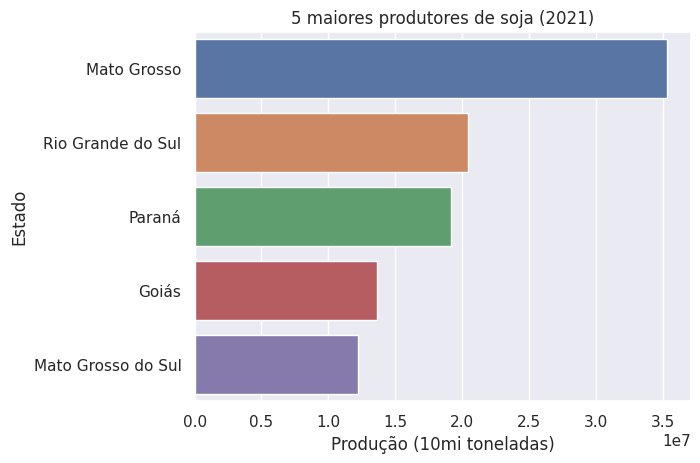
\includegraphics[scale=0.6]{top5_prod_soja_br.png}
\end{center}
Olhando para os últimos anos o Mato Grosso sempre apresentou crescimento na produção de soja e no valor total da produção. No ano de 2021 há um descasamento entre o volume produzido e o valor, isso ocorre por conta do aumento de um \textbf{choque negativo de oferta} por conta dos efeitos da pandemia da Covid que travaram as cadeias produtivas levando à uma alta de preços.
\\~\\
O primeiro caso de Covid-19 reportado em Wuhan foi em dezembro de 2019, porém estudos apontam que os primeiro casos provavelmente datam de novembro\footnote{fonte: https://journals.plos.org/plospathogens/article?id=10.1371/journal.ppat.1009620}, além disso, sabemos que a China é uma autocracia e não podemos confiar muito nos dados divulgados.
\\~\\
Outro fator importante para o mercado de soja é o agravamento da Guerra Russo-Ucraniana com a Batalha de Kiev iniciada em fevereiro de 2022. Na data atual (13/01/2022) o Instituto Brasileiro de Geografia e Estatística (IBGE) ainda não disponibilizou os dados concretizados da produção de 2022 para um análise mais adequada de como o conflito afeta o mercado de soja brasileiro.
\begin{center}
\includegraphics[scale=0.6]{soja_mt.png}
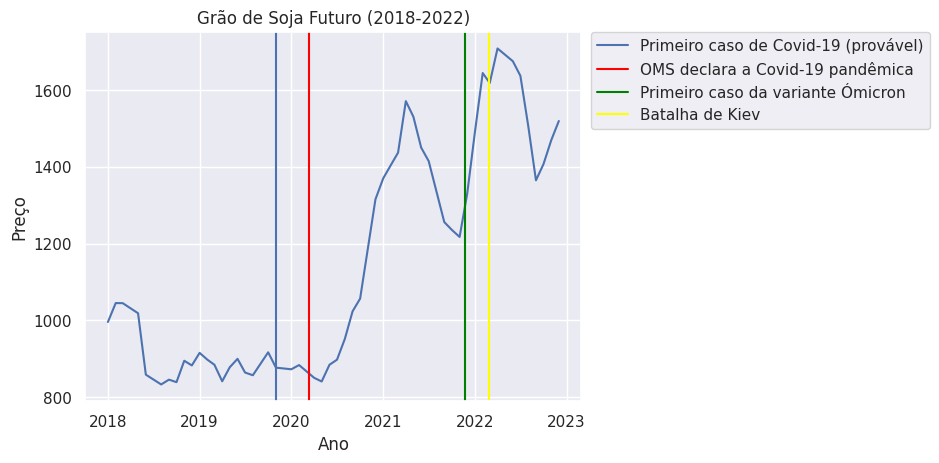
\includegraphics[scale=0.6]{soja_futuro.png}
\end{center}
\section*{O Mercado no Mato Grosso}
No cenária hipótico da abertura de um empresa fertilizantes no Mato Grosso precisamos responder algumas perguntas: 1) "qual o objetivo da empresa?", 2)"qual o indicador correto?", e, 3) "como é o mercado local?".
\\~\\
A primeira pergunta depende do estágio em que a empresa encontra-se, se estamos falando de um empresa nova devemos focar no \textit{marketshare} dela, se falamos de uma filial de uma companhia já consolidada no mercado o foco deve ser na geração de caixa.
\\~\\
Assumindo que seja o primeiro caso, considerando o marketshare precisamos levar em conta o volume produzido pela cidade. As 10 cidades mato-grossences que mais produziram soja em 2021 foram:
\begin{multicols}{2}
\begin{tabular}{|l | r|}
\hline
            Município &     \parbox[t]{2cm}{Volume \\ (Toneladas)} \\ \hline
              Sorriso &                        		 2.010.960 \\
           Nova Mutum &                         1.337.280 \\
              Sapezal &                         1.319.731 \\
           Diamantino &                         1.315.239 \\
   C. Novo do Parecis &                         1.304.958 \\
         Nova Ubiratã &                         1.301.915 \\
            Querência &                         1.298.304 \\
             Canarana &                         1.053.000 \\
   		  P. do Leste &                           939.600 \\
            Brasnorte &                           851.453 \\ \hline
	            TOTAL &                        12.732.440 \\ \hline
\end{tabular}
\columnbreak
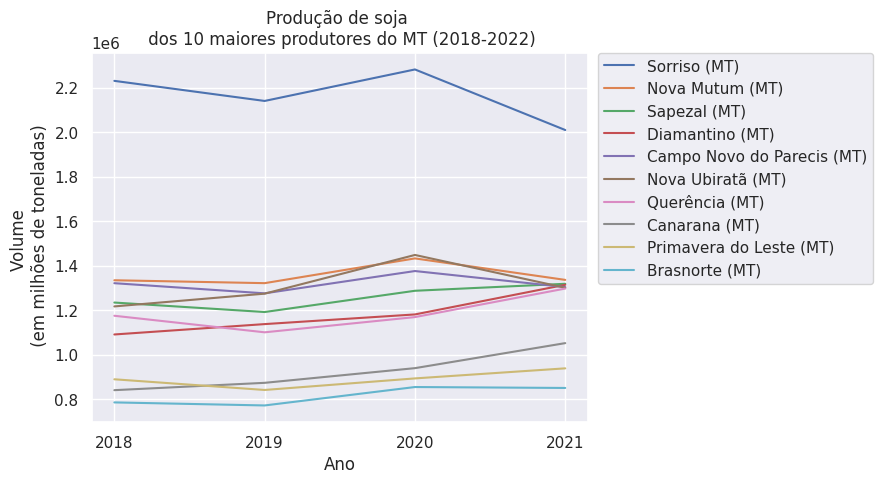
\includegraphics[scale=0.5]{top10_soja_mt_hist.png}
\end{multicols}

\end{document}